\chapter{Biological Background} 
\label{chap:BioFound}
This chapter gives a short overview of the biological foundations, as a background for non-biologists from the view of a computer scientist, to understand the algorithms and applications presented in this thesis, by covering all relevant biological aspects in a simple manner. Due to the fact that the mitochondrial genome sequence is fully decoded since 1981 by Anderson \cite{Anderson1981} and corrected later in 1999 by Andrews et al. \cite{Andrews1999} to the revised Cambridge Reference Sequence (rCRS) with 16569 bases, its analysis has matured in the course of the past 20 years \cite{BandeltHansJurgenRichardsMartinMacaulay2006}. Since then the importance of mtDNA gained, now widely being used for population genetics, forensic DNA fingerprinting and clinical disease association studies \cite{Weissensteiner2010}. In this work the focus is on software tools for human evolution (haplogroups) and disease (haplogroups, heteroplasmy), at first sight appearing unrelated, but the evidence increases that the evolution of mtDNA can have a role in disease expression\cite{BandeltHansJurgenRichardsMartinMacaulay2006}. 

\section{Mitochondrial DNA}
Mitochondrial DNA, which is the data being managed in this thesis, is a sequence of 16.6 kilobases in length (kb), consisting of 4 nucleobases, namely adenine (A), cytosine (C), guanine (G) and thymine (T). The mitochondrial genome is most likely the result of an endosymbiotic process, indicated by the similarity to bacterial (prokaryotic) DNA \cite{Pittis2016}, being circular (see Figure \ref{fig:rcrs}, differing significantly from nuclear DNA (see Table \ref{tab:features}) and showing codons, that differ from the nuclear ones (see Table \ref{tbl:aac}. 
\begin{figure}[ht]
\begin{center}
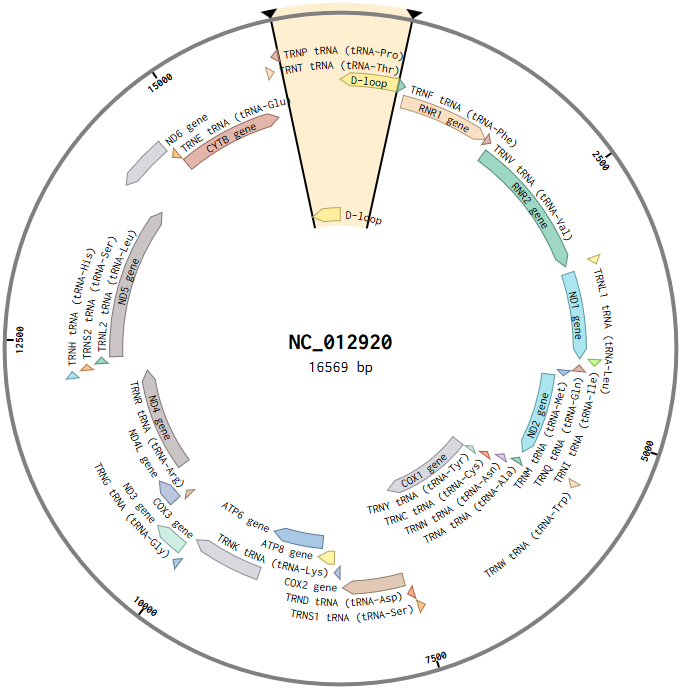
\includegraphics[scale=0.5]{rcrs.png}
\caption[Genomic organization of human mtDNA]{Genomic organization of human mtDNA. }
\label{fig:rcrs}
\end{center}
\end{figure}
It is a circular, double stranded molecule, whereat cytosine binds to guanine and adenine to thymine. One of the two strands is a guanosine-rich "`heavy"' strand (H-strand), the other a cytosine-rich "`light"'strand (L-strand). This is due to the fact that purines (adenine and guanine) are heavier than the pyrimidines (thymine and cytosine) due to their extra ring, see Figure \ref{fig:figureBases}.
\begin{figure}[ht]
\begin{center}
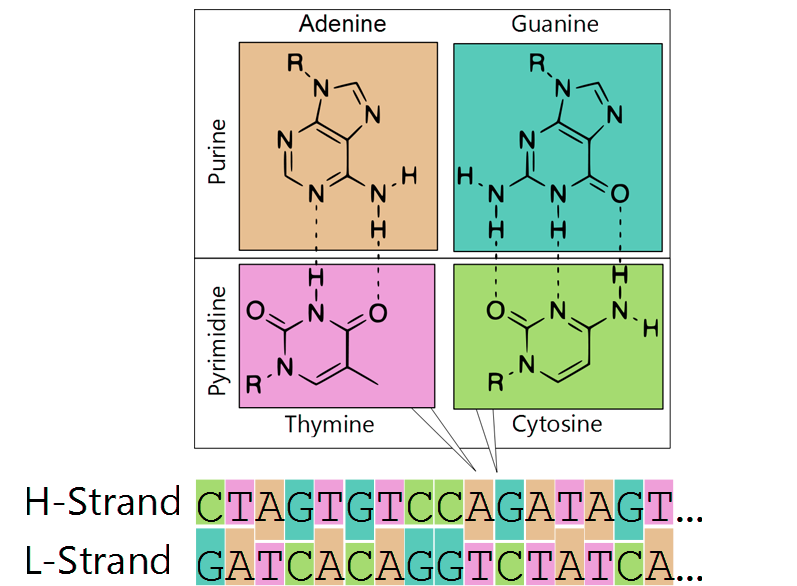
\includegraphics[scale=0.3]{bases2.png}
\caption[Nucleobases binding to a sequence]{Nucleobases binding to a sequence. For convenience only the L-strand is used as the reference sequence (here the first bases of the rCRS), since the H-strand is the complement that can be derived from this sequence.}
\label{fig:figureBases}
\end{center}
\end{figure}

The human mtDNA is numbered according to the light-strand, based on the original Cambridge Reference Sequence \cite{Anderson1981}. This reference sequence contained some major errors (10 substitution errors and a deletion), but to avoid confusion the authors of the revised CRS (rCRS) \cite{Andrews1999} kept the original light-strand numbering system by introducing a base N (for any) to keep the numbering with older analyses consistent. Behar et al. \cite{Behar2012} introduced an artificial new reference sequence, the so called Reconstructed Sapiens Reference Sequence (RSRS), however being kept consistent with the numbering. This was not the case with the Genome Reference Consortium build 36 \footnote{\url{https://genome.ucsc.edu/FAQ/FAQreleases.html}} by using a Yoruba individual (YRI) sequence which due to insertions and deletions (indels) led and still leads to confusion among researchers. The reference was removed \footnote{\url{http://www.ncbi.nlm.nih.gov/nuccore/NC_001807.4}} from the main public database by the National Center for Biotechnology Information (NCBI) \footnote{\url{http://www.ncbi.nlm.nih.gov/}}. Throughout this work the rCRS represents the reference sequence used. 
\begin{table}[ht]
  \begin{tabular}{lll}
     \toprule
    feature  & mtDNA & nDNA \\ 
		\midrule
    size & 16.6 kb & 3.2 Gb  \\ 
		chromosomes & 1 & 22 pairs + XY (male) or XX (female)\\ 
    inheritation & maternal line & recombination (not for Y chromosome) \\ 

		genes & 13 & $\sim$ 20,000\footnote{\url{https://academic.oup.com/hmg/article-lookup/doi/10.1093/hmg/ddu309}} \\ 
		copies per cell & 100-10,000 & 2 \\ 
		\bottomrule
    \end{tabular}
    \caption[Comparison overview mtDNA and nDNA]{Comparison overview of mitochondrial and nuclear DNA }
    \label{tab:features}
\end{table}

\begin{figure}[ht]
\begin{center}
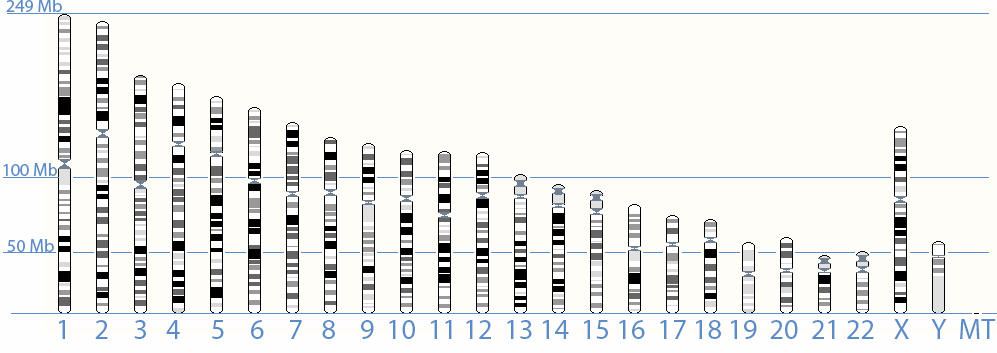
\includegraphics[width=\textwidth]{chromosomes.png}
\caption[Chromosome size comparison]{Chromosome size comparison. Although mtDNA is only $\sim$ 17 kb, due to its high copy number per cell amounts to approximately 0.1\% to 1\% of the total DNA.}
\label{fig:figureChromosomes}
\end{center}

\end{figure}

\section{Data generation}
\label{sec:dataGeneration}
To attain the informations in the mitochondria respectively their DNA, generally two different approaches exist, being the same as for the nuclear DNA (short nDNA). One approach is to read the whole sequence or a smaller part of it, the other is to look at very specific positions, so called single nucleotide polymorphisms (SNP) of an already known sequence. The technical terms for the two approaches are sequencing and genotyping and are drafted in the following subsections.
\subsection{Sequencing}Due to the special properties of the mtDNA sequences, often only the non-coding displacement loop (D-Loop) or control region (CR) with about 1 kilobases (kb) is sequenced, this is especially the case in forensics, where it is even more restrictive to the hypervariable regions 1 and 2 (HVI + HVII) depending on the law policy in the different countries. In clinical studies the whole 16.6 Kb sequence is mostly analyzed, since 93.2\% of the nucloetides are in the coding region, responsible for the encoding of the 13 genes to proteins, 22 genes to tRNAs and 2 genes to rRNAs\cite{Sosa2012}. The method used for reading out the mtDNA nucloetides string, is the same as for nucleotide DNA. It has been established by Nobel Laureate Frederick Sanger and colleagues, and is therefore referred to as Sanger Sequencing. The principle idea of this method is essentially the same as happens in nature by replicating the DNA by the enzyme DNA polymerase.
The exception is that an additional `dummy' nucleotide - dideoxynucleotide triphosphate - gets incorporated in the growing DNA chain, causing the reaction to terminate. This reaction can be seen by gel electrophoresis and the incorporated base can be determined. So each incorporation of these dideoxynucleotides (dideoxy ATP or ddATP, ddCTP, ddGTP and ddTTP) terminates at different positions yielding to the final sequence on the autoradiogram.
This method was improved over the years, by using robots running the sequencing reactions and lasers to scan the gel and finally computers to interpret the generated data \cite{WallaceRobertA.SandersGeraldP.1996}. As result we get the whole or partial sequence in a text file, the so called FASTA format after the electropherograms are checked by two different scientists or lab members\cite{Weissensteiner2010}. See figure \ref{fig:figureElectro} for an example of how this data is represented. 
\begin{figure}[ht]
\begin{center}
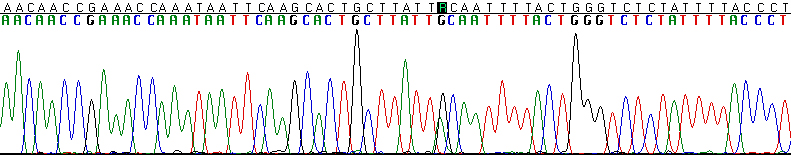
\includegraphics[scale=0.46]{electro9702.png}
\caption[Representation of an electropherogram]{Partial representation of an electropherogram in the Software Sequencher, showing an heteroplasmy on the overlapping curves denoted by R.}
\label{fig:figureElectro}
\end{center}
\end{figure}
\newline
A FASTA file begins with the first line containing the symbol \verb|">"| followed by the identifier with no space in between. In the next lines, the nucleotide sequence is provided, where each nucleotide is represented with the initial one-letter abbreviation (nucleic acid code) for \verb|A|denine, \verb|G|uanine, \verb|C|ytosine and \verb|T|hymine. See listing  \ref{lst:fasta} for an example mtDNA sequence file\footnote{the authors mtdna sequence \url{http://www.ncbi.nlm.nih.gov/nuccore/301505865}}. Some special characters exist, like \verb|N| for aNy, \verb|Y| for pYrimidines or \verb|R| for puRine, besides others. In the mitochondrial context, this way heteroplasmies can be described. A FASTA file can also contain alignment characters represented by \verb|"-"|,  or contain amino acid sequences as for protein or peptide sequences with their own amino acid code. Table \ref{tbl:aac} lists the 20 amino acids translated by the corresponding triplets of nucleotides, called codons.
\newline
{\small 
\begin{lstlisting}[caption= {Excerpt of an mtDNA fasta file, here the first 350 bases of 16,570}, label={lst:fasta}]
>gi|301505865|gb|HM625680.1| Homo sapiens isolate Lab003 mitochondrion
GATCACAGGTCTATCACCCTATTAACCACTCACGGGAGCTCTCCATGCATTTGGTATTTTCGTCTGGGGG
GTATGCACGCGATAGCATTGCGAGACGCTGGAGCCGGAGCACCCTATGTCGCAGTATCTGTCTTTGATTC
CTGCCTCATCCTATTATTTATCGCACCTACGTTCAATATTACAGGCGAACATACTTACTAAAGTGTATTA
ATTAATTAATGCTTGTAGGACATAATAATAACAATTGAATGTCTGCACAGCCGCTTTCCACACAGACATC
ATAACAAAAAATTTCCACCAAACCCCCCCTCCCCCCGCTTCTGGCCACAGCACTTAAACACA...
\end{lstlisting}
}
\begin{table}[ht]
\begin{tabular}{lccl}
\textbf{Amino Acid}&\textbf{3-Letter}&\textbf{1-Letter}&\textbf{Codon}\\ 
\hline
Alanine&Ala&A&GCA GCC GCG GCT \\ 
Arginine&Arg&R&CGA CGC CGG CGT \\ 
Asparagine&Asn&N&AAC AAT\\ 
Aspartic acid&Asp&D&GAC GAT \\ 
Cysteine&Cys&C&TGC TGT \\ 
Glutamine&Gln&Q&CAA CAG \\ 
Glutamic acid&Glu&E&GAA GAG \\ 
Glycine&Gly&G&GGA GGC GGG GGT \\ 
Histidine&His&H&CAC CAT \\ 
Isoleucine&Ile&I&\underline{ATC} \underline{ATT} \\ 
Leucine&Leu&L&CTA CTC CTG CTT TTA TTG\\ 
Lysine&Lys&K&AAA AAG \\ 
Methionine&Met&M&\textbf{\underline{ATA}} \underline{ATG}\\ 
Phenylalanine&Phe&F&TTC TTT \\ 
Proline&Pro&P&CCA CCC CCG CCT \\ 
Serine&Ser&S&AGC AGT TCA TCC TCG TCT\\ 
Threonine&Thr&T&ACA ACC ACG ACT \\ 
Tryptophan&Trp&W&\textbf{TGA} TGG \\ 
Tyrosine&Tyr&Y&TAC TAT \\ 
Valine&Val&V&GTA GTC \underline{GTG} GTT  \\ 
Terminating codon&&&\textbf{AGA} \textbf{AGG} TAA TAG \\ 
\end{tabular}
\caption[Vertrebrate mtDNA genetic code]{Vertrebrate mtDNA genetic code: 20 Amino Acids translated from the codons. Codons in bold differ from the "Universal" code, underlined codons represent Start-codons. }
\label{tbl:aac}
\end{table}
As represented in the table \ref{tbl:aac}, each of the 13 protein coding genes in the mtDNA, start with either Isoleucine, Methionine or the Valine triplet GTG and are terminated by the triplets in the last row. The listing \ref{lst:fastaAAC} shows the amino acid sequence of the ATP-6 gene\footnote{\url{http://www.ncbi.nlm.nih.gov/protein/ADK77199}}, which starts on position 8527 according to the rCRS so that the first triplet is ATG corresponding to Methionine, represented by M in the protein sequence.
{\small 
\begin{lstlisting}[caption= {Example of a FASTA protein sequence - here the complete ATP-6 gene}, label={lst:fastaAAC}]
>gi|301505871|gb|ADK77199.1| ATP synthase F0 subunit 6 (mitochondrion)
MNENLFASFIAPTILGLPAAVLIILFPPLLIPTSKYLINNRLITTQQWLIKLTSKQMMTMHNTKGRTWSL
MLVSLIIFIATTNLLGLLPHSFTPTTQLSMNLAMAIPLWAGAVIMGFRSKIKNALAHFLPQGTPTPLIPM
LVIIETISLLIQPMALAVRLTANITAGHLLMHLIGSATLAMSTINLPSTLIIFTILILLTILEIAVALIQ
AYVFTLLVSLYLHDNT
\end{lstlisting}
}
The sequence data of published mtDNA is mainly stored in Genbank\footnote{\url{http://www.ncbi.nlm.nih.gov/genbank/}} \cite{Benson2005}, the NIH genetic sequence database. The search term in listing \ref{lst:genbankquery} , yields currently\footnote{as of October 2016} 32,248 homo sapiens sequences, including 12 homo sapiens neandertalensis and 4 homo sapiens subspecies Denisova. 
The correctness of this data is not always given, and has to be handled with precaution. Quality control mechanisms are therefore needed and solutions are presented in chapter \ref{chapterHaplogrep}. 
\begin{lstlisting}[caption={GenBank queries for mtDNA sequences}, label={lst:genbankquery}]
//Homo sapiens
(("Homo sapiens"[Organism] OR Homo sapiens[All Fields]) AND mitochondrion[All Fields] AND complete[All Fields] AND genome[All Fields]) AND "Homo sapiens"[porgn]
//Homo sapiens neanderthalensis
(("Homo sapiens"[Organism] OR Homo sapiens[All Fields]) AND mitochondrion[All Fields] AND complete[All Fields] AND genome[All Fields]) AND "Homo sapiens neanderthalensis"[porgn] 
//Homo sapiens Denisova
Homo sapiens ssp. Denisova 
\end{lstlisting}
\subsection{Genotyping}
In contrast to the previously described method of mtDNA sequencing, genotyping is the process of determining a specific position on a known DNA sequence. Positions of interest are so called single nucleotide polymorphisms (SNPs) as the most common form of genetic variation between individuals\cite{Perkel2008}. The concept of genotyping is to use the known region prior and behind the SNP as so called primers, that bind on the DNA. SNPs were estimated to occur at 1 out of every 1,000 bases on the nuclear DNA \cite{Syvanen2001} in 2001. While in 2008 over 12.8 million SNPs were present in the free public archive Single Nucleotide Polymorphism Database (dbSNP)\footnote{\url{https://www.ncbi.nlm.nih.gov/books/NBK44423/}}, there are about 88 million SNPs present in the 1000 Genome Phase 3 data \cite{Auton2015}, based on 2,504 samples. The work thereby represents DNA composition in 26 populations around the world. 39 million SNPs can be found in European populations, as investigated by the Human Reference Consortium \cite{McCarthy2016} in 2016, based on 30,000 samples. There are about 1,680 SNPs (mtSNPs) on the mitochondrial genome, to be found through Ensembls \cite{Flicek2014} Biomart\footnote{\url{http://www.ensembl.org/biomart/martview/} release Ensembl Variation 86 (GRCh38.p7)}. In over 38 million SNPs provided by the 1000 Genomes Project Consortium Phase 1 \cite{Abecasis2012} 2,834 mitochondrial SNPs (mtSNPs) can be found on the FTP Server\footnote{\url{ftp://ftp.1000genomes.ebi.ac.uk/vol1/ftp/phase1/analysis_results/integrated_call_sets/}}. Figure \ref{fig:figureSNPlocation} represents the SNPs over the mitochondrial genome. When further looking at the rare mtSNPs used for the mitochondrial phylogeny in Phylotree \cite{VanOven2009},\cite{VanOven2010} in the current release 17 based on 24,275 sequences $\sim$ 4,560 different variants or 3,740 transitions, 399 transversions, 50 inserts, 50 deletions and 123 back mutations defining and 5,435 haplogroups) exist. Some of these genotypes are known to cause severe diseases such as Leber hereditary optic neuropathy (LHON\footnote{[OMIM 535000] \url{http://omim.org/entry/535000}}) being the most common mtDNA disease leading to blindness. It is caused by one of three mtSNPs 3460A, 11778A, and 14484C in 95\% of all cases \cite{Elson2007}. With technical improvements, the calling of genotypes is performed on platforms like the Sequenom Platform, allowing to genotype 40 SNPs in a sample set of 396 in one run\cite{Weissensteiner2013}, or on a MicroArray per sample, allowing to detect up to 5 million SNPs  \footnote{\url{http://www.illumina.com/Documents/products/datasheets/datasheet_gwas_roadmap.pdf}}, where up to 4,000 mitochondrial variants\footnote{\url{https://www.livingdna.com/en-gb/help-centre/87/what-technology-behind-procedure}} are included.

\begin{figure}[ht]
\begin{center}
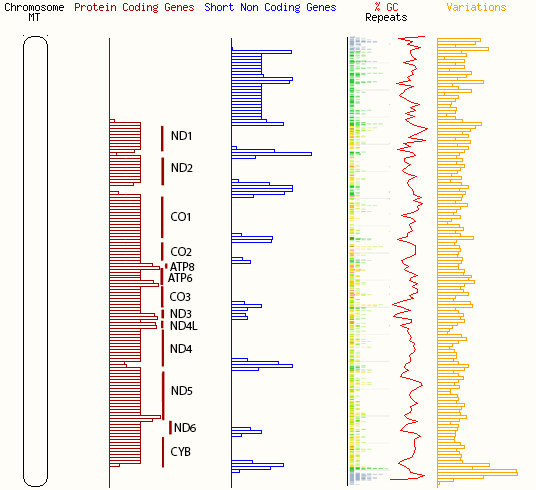
\includegraphics[scale=0.7]{ensembl_mt2.png}
\caption[mtSNPs location on mtDNA]{Overview of the mtSNPs and their location on the mtDNA. Figure modified from UCSC Genome Browser\footnote{\url{https://genome-euro.ucsc.edu/index.html}}}
\label{fig:figureSNPlocation}
\end{center}
\end{figure}

\subsection{Next Generation Sequencing (NGS)}
The step from conventional Sanger Sequencing to NGS revolutionized the genomics research area, however it came also with two shortcomings for the latter: read length was very short (about 36 base pairs\cite{Li2013a} in the beginning compared to 1,000 base pairs in Sanger) and the error rate a tenfold higher. New algorithms were required for assembling the short reads to a reference genome (called mapping) if already available or to a de-novo sequence, in the case no reference sequence can be used. The big advantage of NGS over Sanger Sequencing is the amount of data throughput (several hundred Gigabases per Run instead of some Kilobases), the speed and the much lower cost per base. Hundreds of mtDNA samples can be processed in one run, by generating high-coverage mtDNA sequences. 
The classical FASTA format was extended to so called FASTQ files, where besides the nucleotide sequence also their quality scores are stored as ASCII characters (see Data description \ref{datadescription}). Additional files for storing the mapping as well as for the called variants are now de facto standards, and are presented within this subsection. 
\section{Data description}\label{datadescription}
With almost every sequencing-device vendor having its own file format, the first step after a successful run, is the conversion of the primary analysis results in form of images of some terabites to its own fasta like sequencing file. There are different FASTQ file encoding (Sanger, Solexa, Illumina), Color Space Fasta files (.csfasta for ABI SOLiD) or Standard Flowgram Files (SFF for Roche and Ion Torrent). The raw FASTQ files need to be mapped to a reference sequence in order to compare the results and based on this mapping, the variant calling can be performed, yielding to VCF files. The next subsections represent the data and how it is structured. 
\subsection{Raw Reads: FASTQ file}
For the described application in Chapter \ref{chap:NGS}, the  direct support of FASTQ files of different encodings is required. SFF (by Roche) and color space (csfasta, by Thermo Fisher Scientific) files, besides others\footnote{\url{https://www.ncbi.nlm.nih.gov/sra/docs/submitformats/}} can be converted straight forward to FASTQ, which nowadays is the standard format for NGS results.  
Listing \ref{lst:fastq} shows the structure of a FASTQ file. 4 rows characterize one read. This has to be taken into consideration, as shown in Chapter \ref{chap:NGS}, when splitting up files at fixed sizes as it is the case in MapReduce with its 64 MB blocks. Listing \ref{lst:fastq} depicts the structure, where the first row indicates the read-number, the second row represents the actual nucleotide sequence, the third row is optional and mostly consisting of the symbol {+} only and the fourth row represents the base quality, encoded in ASCII code. So the first nucleobase G with ! as ASCII character has numerical value of 33 being the first printable code, the base A has value 39 (') see  ASCII Codes Table\footnote{\url{http://ascii.cl/}}. Read length varies usually between dozens to some hundred bases (e.g. for Ion Torrent depending on chemistry up to 400 base pairs) or can be a fixed length (101 nucleotides for the Illumina HiSeq). Depending on the device data can be so called single- or paired end. In contrast to single-end, paired-end sequencing is characterized by 2 resulting FASTQ files per sample, where reads from both files are checked based on their read number and provide a much higher accuracy and are more likely to map to a reference\footnote{\url{http://technology.illumina.com/technology/next-generation-sequencing/paired-end-sequencing_assay.html}} since the reads come from the same fragment from both ends.
\begin{lstlisting}[caption= {Excerpt of an FASTQ file, 4 rows representing one read}, label={lst:fastq}]
@SEQ_ID
GATTTGGGGTTCAAAGCAGTATCGATCAAATAGTAAATCCATTTGTTCAACTCACAGTTT
+
!''*((((***+))%%%++)(%%%%).1***-+*''))**55CCF>>>>>>CCCCCCC65
\end{lstlisting}
\subsection{Aligned reads: BAM file}
Besides the previously presented "`raw"' sequence format, some defacto standards in the NGS environment are presented in this paragraph. The most established being the Sequence Alignment/Map (SAM) format \cite{Li2009} supporting single- and paired-end reads. It can include different raw formats not only FASTQ, such as the before mentioned color space reads. The format consists of 2 sections for header and alignment informations. Header content is characterized by "`@"' symbol, the alignment informations are tab delimited and require 11 mandatory fields. Listing \ref{lst:sam} shows an example SAM file\footnote{\url{http://samtools.github.io/hts-specs/SAMv1.pdf}} 
\begin{lstlisting}[caption= {Excerpt of a SAM file, representing two reads}, label={lst:sam}]
@HD VN:1.5 SO:coordinate
@SQ SN:ref LN:45
r001 99 ref 7 30 8M2I4M1D3M = 37 39 TTAGATAAAGGATACTG *
r002 83 ref 9 30 3S6M1P1I4M *  0  0 AAAAGATAAGGATA    *
\end{lstlisting}
The CIGAR string in column 6 (for r001: 8M2I4M1D3M) represents the read and it's operations needed to be mapped to a reference string. The operations are M for Match, I for Insertion, D for Deletion and S for Substitution. 
The quality scores are the same as in the FASTQ file, given as Phred-scaled quality values where $\left( Q=-10\log_{10} P\right)$ where $P$ is the probability that the base call is correct\cite{Loman2012}. Additionally TAGs in the form of key value pairs can be provided in the last column, however in the example not used (denoted by the symbol *).
A BAM file is the binary representation of a SAM file, hence much smaller in filesize. Both SAM and BAM files have an Index (called .sai or .bai respectively), and are sorted, so that direct access to a region of interest is guaranteed and not the whole file has to be processed. This is of special interest when downloading of a small region like the mitochondrial genome covered in a Whole Genome Sequencing run should be carried out. Instead of downloading about 120 GB (for a high-coverage whole-genome experiment with coverage ~40x) per sample, only approx. 100MB are downloaded (depending on the mitochondrial copy number present in the sample).
\subsection{Variants: VCF file}\label{intro:VCF}
To get the specific mutations from a BAM file, a variant calling step is required. There are many tools available to perform this step, and provide a VCF file, where the results per sample and per position on the DNA are listed. The strucutre of the VCF files is maintained by the Global Alliance Data Working Group File Formats Task Team \footnote{\url{http://ga4gh.org/\#/fileformats-team}}. The specifications can be found on the Github page\footnote{\url{https://vcftools.github.io/specs.html}}. Summed up, it is a text file that has meta-information lines about genotype informations before the actual header line which can contain different columns, requiring 8 fixed fields, as represented in Table \ref{table:vcf}. After these fixed columns, Sample Ids can be appended, separated by tab, cotaining the genoptype information ("`GT"') per position, or extended to customized informations such as nucleobases and base count for next-generation sequencing data.

\begin{table}[H]
  \begin{tabular}{lll}
    \toprule
    Field & Description & Example \\
		\midrule
    \#CHROM & Number of Chromosome & MT or chrM \\
    POS & Position of the variant/SNP & 73, 263,.. \\
    ID & ID of the SNP, otherwise "`."' & rs3087742, .\\
    REF & base on reference & A, A, ...\\
    ALT & transition/transversion & G, G,C...\\
    QUAL & quality as phred score & 50 \\
    FILTER & all filters passed & PASS \\
    INFO & additional information & CIGAR \\
		\bottomrule
\end{tabular}
\caption{Fixed fields in an VCF file, the new standard format for called variants}
\label{table:vcf}
\end{table}